\documentclass[aip, jcp, reprint, onecolumn]{revtex4-2}

\bibliographystyle{apsrev4-2}

\usepackage{physics}
\usepackage{amsmath}
\usepackage{amssymb}
\usepackage{mathtools}
\usepackage{graphicx}
\usepackage{dcolumn}
\usepackage[colorlinks=true, linkcolor=black, urlcolor=blue, citecolor=black, anchorcolor=black]{hyperref}

\graphicspath{{"figures/"}}
\begin{document}
%Title of paper
\title{Coherent IR-Hyper-Raman Four Wave Mixing Spectroscopy}


\author{Ryan P. McDonnell} 
\author{Daniel D. Kohler}
\author{John C. Wright} \email{wright@chem.wisc.edu}

\affiliation{Department of Chemistry, 
        University of Wisconsin - Madison, 
        Madison, Wisconsin 53706, 
        United States of America}

\date{\today}

\begin{abstract}
Nonlinear, four wave mixing vibrational spectroscopies are commonly used to probe electron-vibration coupling in isotropic media.
Most of these methods rely on infrared and/or Raman transitions, but methods involving hyper-Raman transitions are also possible. 
Hyper Difference Frequency Generation (HDFG) spectroscopy is an underdeveloped four wave mixing vibrational spectroscopy based on the hyper-Raman transition and IR absorption. 
HDFG is experimentally similar to vibrational sum frequency generation (vSFG) spectroscopy share similar output, making HDFG feasible for vSFG practitioners. 
Despite several experimental reports on HDFG, its spectroscopic properties have not been fully explored. 
To this end, we investigate the selection rules and behavior of HDFG spectroscopy as an upconverted infrared spectroscopy and as a probe of vibronic coupling in molecular systems.
HDFG is shown to a sensitive probe of vibronic coupling in bulk systems.
\end{abstract}

\maketitle

\section{Introduction}
Coherent multidimensional spectroscopy (CMDS) is a family of nonlinear spectroscopy methods that form the optical analogue of multidimensional nuclear magnetic resonance (NMR) spectroscopy.\cite{Cho2008}
Multiresonant, four wave mixing CMDS experiments, first proposed by Oudar and Shen in 1980,\cite{RN307} directly probe coupling and correlations between different vibrational, electronic, and vibronic states. \cite{RN281, RN103, Cho2008} 
Four wave mixing CMDS has resolved anharmonicities, ultrafast dynamics, and other inter- and intra-molecular couplings in numerous systems. \cite{Cho2008, Gaynor2017, Ziegler2018, Ogilvie2019, Bonn2021, RN325, Chen2024}
To target vibrational and electronic coupling, methods commonly make use of Raman transitions, e.g., doubly vibrationally enhanced spectroscopy (DOVE), triple sum frequency (TSF), coherent anti-Stokes Raman spectroscopy (CARS), resonant impulse stimulated Raman spectroscopy (RISRS).\cite{RN103, Dhar1994, RN345, Cho2000, RN491}
Here we explore the less-utilized hyper-Raman transitions in four wave mixing CMDS.

\begin{figure*}[!htbp]
	\centering
	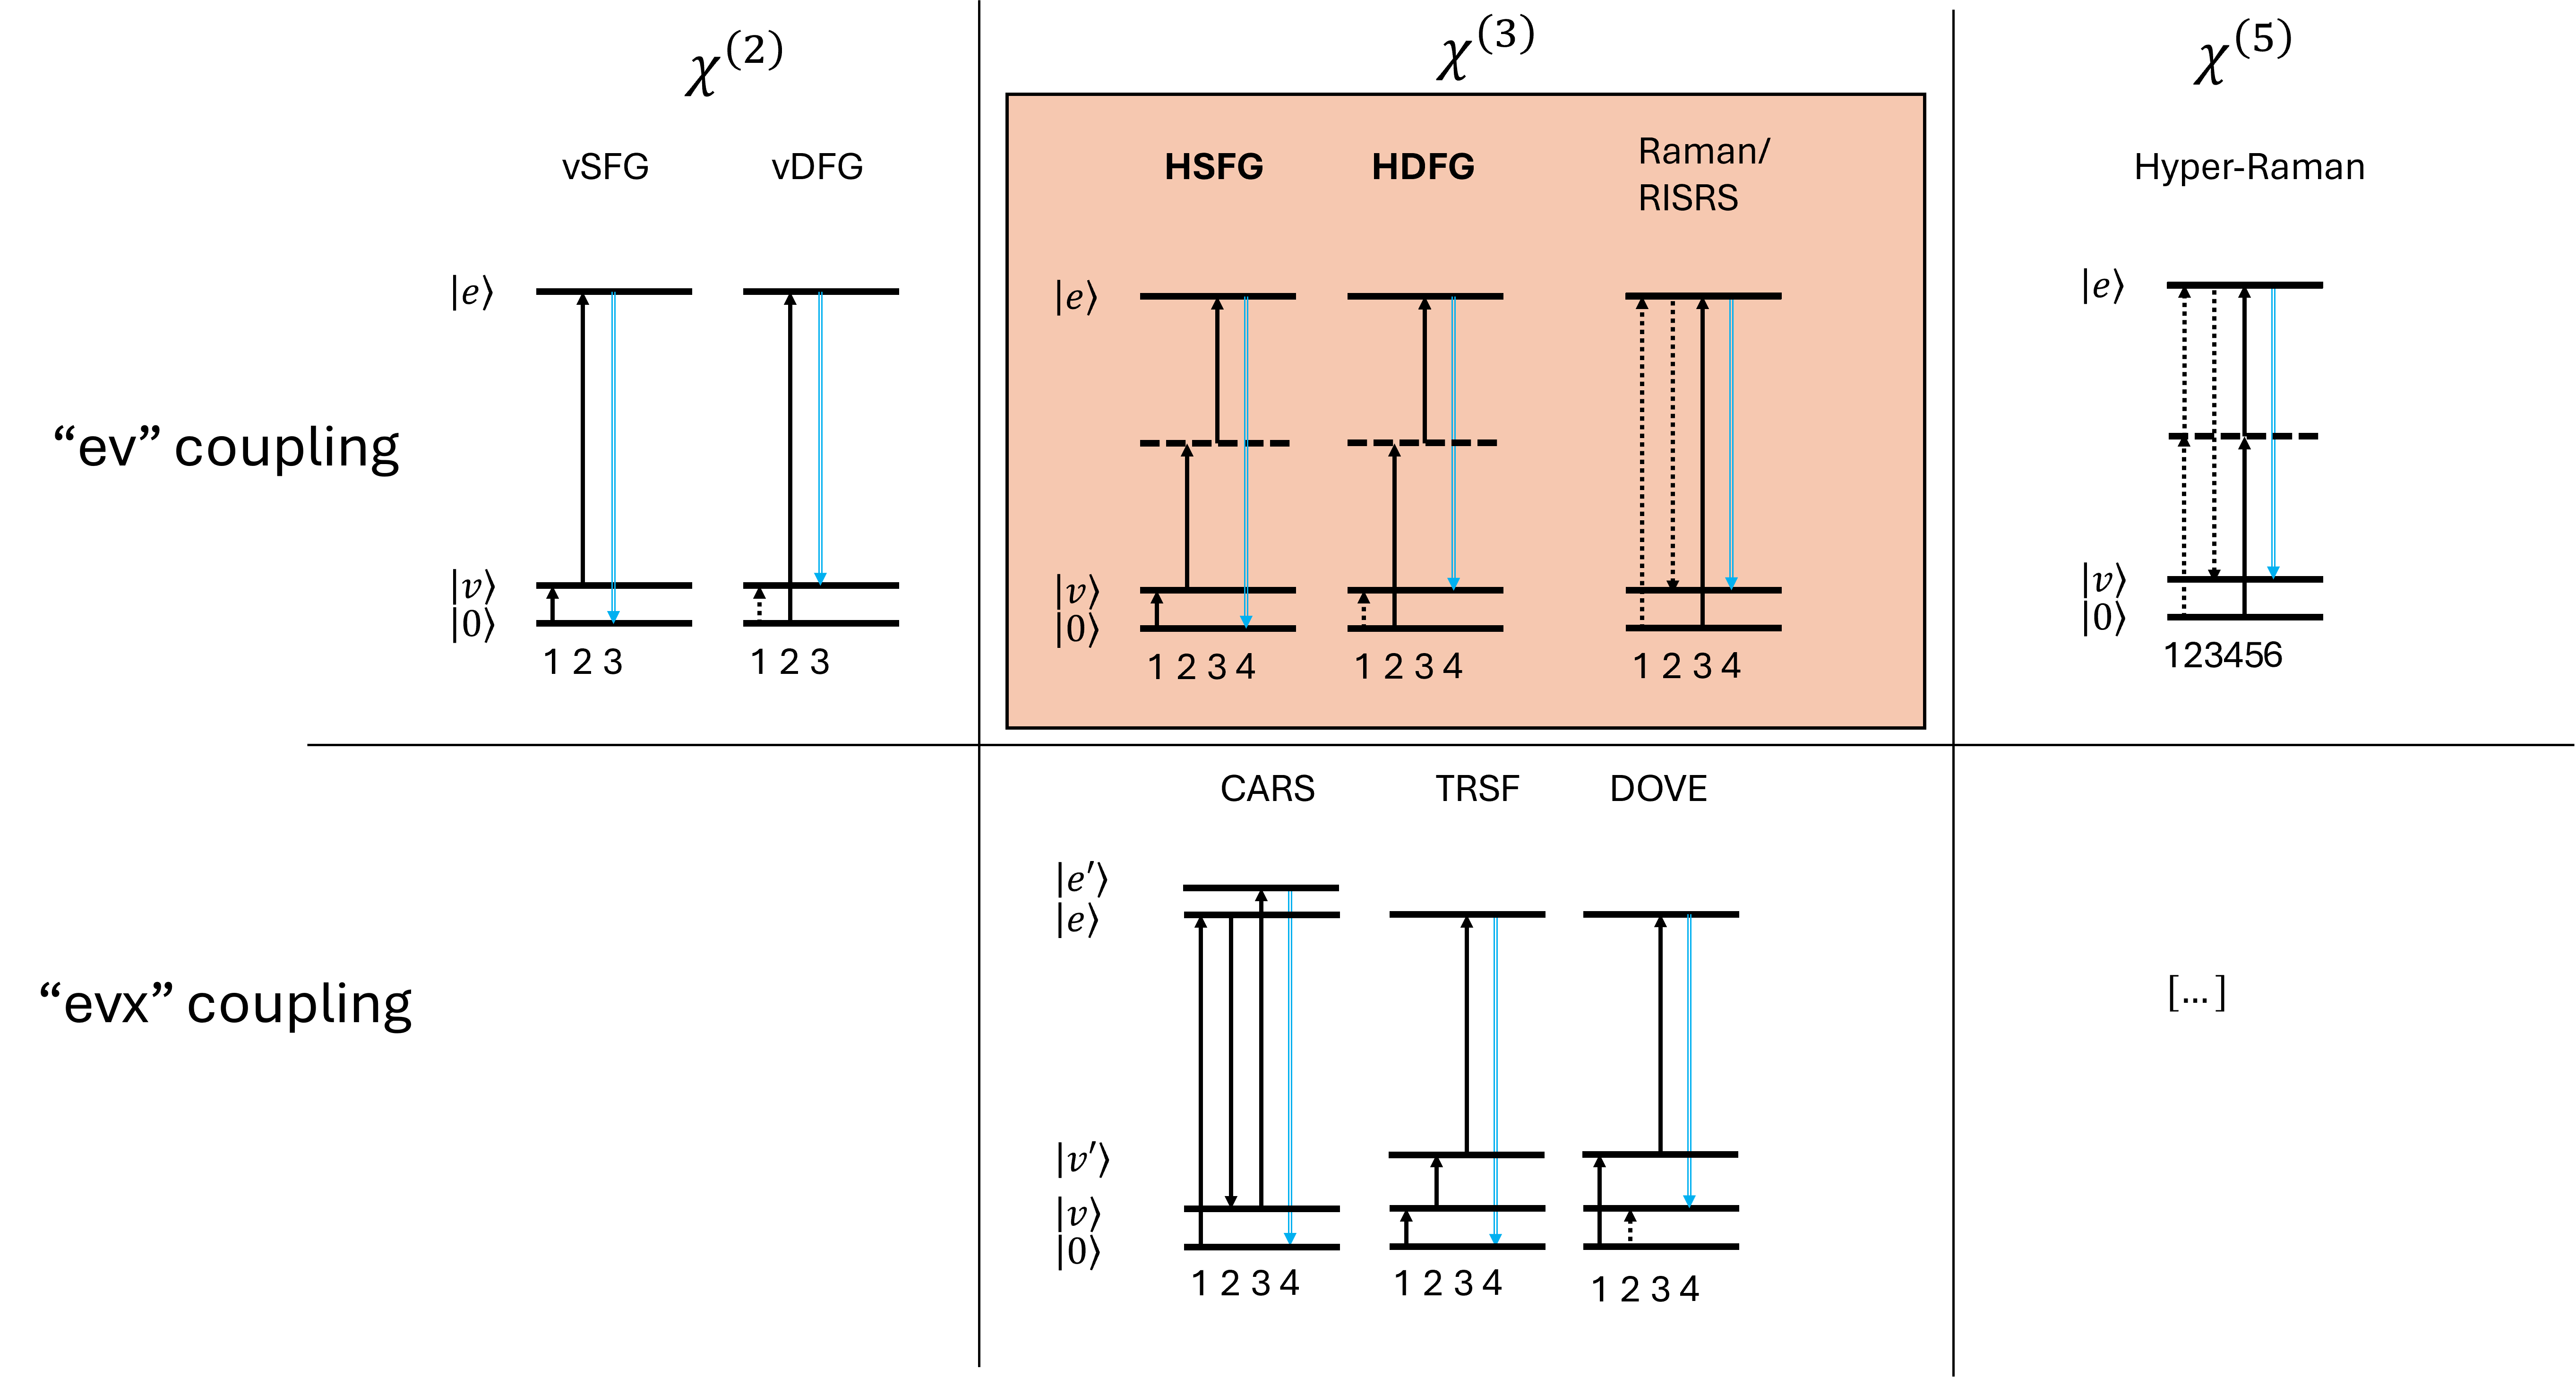
\includegraphics[width=6.66in]{taxonomy.png}
	\caption{
		Some spectroscopic methods for investigating (top) electronic-vibrational coupling and (bottom) e-v-x (x: e, v, e-v, e-v-e) coupling through different order nonlinear processes.
		The light-matter interactions are depicted using Wave Mixing Energy Level (WMEL) diagrams.\cite{RN286}
		Solid and dashed horizontal lines indicate real and virtual states, whereas solid and dotted arrows indicate ket and bra side transitions, respectively. 
		The red box outlines the e-v coupling techniques (HDFG, HSFG) relevant to this manuscript.
	} %TODO: Fix vsfg
	\label{fig:comparisonwmel}
\end{figure*}

The hyper-Raman transition is the nonlinear, two photon analogue to the Raman transition.\cite{Terhune1965, Cyvin1965, Andrews1978}
Two photons of frequency $\omega_a$ and $\omega_b$ inelastically scatter with matter, promoting or demoting a vibrational mode of frequency $\omega_v$ and emitting a single photon of frequency $\omega_a + \omega_b \mp \omega_v$. 
While most hyper-Raman experiments are performed using degenerate input pulses ($\omega_a = \omega_b$), it is possible to perform the technique with non-degenerate input pulses ($\omega_a \neq \omega_b$). \cite{Denisov1986, Kozich2007}
The single photon emission is a significantly different frequency from the excitation frequencies, making rejection of excitation scatter much easier.
Unlike Raman, all infrared active modes are hyper-Raman active, which allows infrared active modes to be probed through a two-photon inelastic scattering event. \cite{Andrews1978}
One drawback is that hyper-Raman transitions are typically weak compared to their Raman counterparts, even when accounting for the high intensities available to ultrafast pulsed lasers.\cite{RN515, Kelley2010}
CMDS methods partially mitigate this issue because emission is spatially coherent so that all emission is directional and easily collected.
In fact, hyper-Raman transitions have been observed in several CMDS studies (sometimes under the moniker of SIVE).\cite{Zilian1994, RN350, RN416, RN351, RN352, RN353, Chen1998, RN362, RN418, Wang2021, Bonn2024, McDonnell2024}

Hyper difference frequency generation (HDFG) spectroscopy and hyper sum frequency generation (HSFG) spectroscopy are four wave mixing CMDS methods based on direct excitation of a vibrational mode through IR absorption and subsequent scattering to or from the vibrational mode through a hyper-Raman transition.
In HDFG/HSFG, an infrared pulse is resonant with a vibrational mode, while two other excitations stimulate the hyper-Raman scattering process.
The infrared excitation frequency selects the vibrational modes to be stimulated through the hyper-Raman transition.
The other two excitation frequencies control electronic enhancement for the hyper-Raman scattering event.

\autoref{fig:comparisonwmel} shows both HDFG and HSFG processes and compares them with related spectroscopies that investigate vibrational-electronic coupling.
The three-wave mixing ($\chi^{(2)}$) techniques are often less applicable as they require macroscopic non-centrosymmetry under the electric dipole approximation.\cite{Shen94}
Hyper-Raman scattering itself is a six-wave mixing ($\chi^{(5)}$) technique; stimulated hyper-Raman will be weak and susceptible to four-wave mixing (FWM) cascades.\cite{RN515, RN243, Cho2000_Cascade}
A coherent six-wave mixing analogue of hyper-Raman scattering, coherent anti-Stokes hyper-Raman spectroscopy (CAHRS), has been proposed and explored theoretically by several authors; however, it is also weak and highly susceptible to FWM cascades.\cite{Berger1978, Bjarnason1980, Cho1997, Cho1998}
Of the many four-wave mixing techniques, HDFG and HSFG have strong similarity to Raman, stimulated Raman, and RISRS in that the electronic state must remove or add a $v$ quantum to the ground state (``ev'' coupling).
With the other four-wave and six-wave mixing techniques (\autoref{fig:comparisonwmel}, second row), the output signal depends on more states than just a single vibrational mode and electronic state (``evx'' coupling).\cite{RN445, RN335} 
As a result, the relationship between the output and vibrational-electronic coupling is more detailed, but also more complicated.
HDFG, HSFG and Raman are more direct probes of electronic-vibrational coupling.
Notably, HDFG and HSFG can be implemented as two-color experiments (with $\omega_2=\omega_3$);\cite{Cho2001} vibrational sum frequency generation (vSFG) or difference frequency generation (vDFG) setups can be trivially reconfigured to perform HSFG or HDFG measurements, respectively, to investigate ev coupling in bulk systems.

When the hyper-Raman excitation in HDFG or HSFG is resonant or near-resonant with electronic states, the brightness of the vibrational feature depends on the vibronic structure of the electronic state.
The electronic spectrum probed in HDFG or HSFG can inform on processes that control ultrafast electronic relaxation in molecular and biological systems in similar ways to resonance Raman.\cite{Cho2001, Bredenbeck2015, Arsenault2021}
Since the selection rules of hyper-Raman scattering differ from Raman scattering, the hyper-Raman excitation spectra give a unique alternative to Raman scattering to understand vibrational spectra, electronic structure and vibronic coupling in molecular systems. \cite{Olson2018}

This paper investigates the microscopic parameters that control HDFG output. \cite{Bonn2024, McDonnell2024}
In \autoref{steadystate}, we first identify the vibrational selection rules. 
The selection rules of electronically-resonant HDFG are then identified through a Herzberg-Teller dipole expansion.
HDFG is found to be allowed in any harmonic system that has infrared active vibrations.
A simple harmonic oscillator model system is used to simulate HDFG spectra and illustrate how the excited state potential energy surface affects the hyper-Raman excitation spectrum.
After developing selection rules, some quantitative aspects of HDFG are discussed in \autoref{quant}.

\section{Selection Rules for HDFG Spectroscopy}\label{steadystate}

In this section, we investigate the properties of HDFG and make the connections between HDFG and hyper-Raman scattering explicit.
HSFG will not be discussed, but the application of our treatment to HSFG is straightforward and the selection rules are similar.
We note that HDFG emission can be phase-matched in media with normal dispersion, while HSFG cannot,\cite{RN278} although experimental strategies can be implemented to minimize phase-mismatch in HSFG experiments. \cite{Kaufman2024}  

It is useful to briefly discuss the impact of time ordering on HDFG output.
Dependent upon the time-ordering schemes, it is possible to eliminate output through destructive interference.\cite{RN287}
While we have only isolated one specific HDFG resonance and time-ordering scheme (\autoref{fig:comparisonwmel}), there are several other pathways which can provide HDFG output. \cite{RN352}
If $\omega_2$ becomes resonant and $\omega_1$ becomes non-resonant, where $\omega_2 > \omega_1$, then other HDFG pathways appear (\autoref{fig:sivewmel2}).\cite{McDonnell2024} 
While the methods in \autoref{fig:sivewmel2} possess identical selection rules to \autoref{fig:comparisonwmel}, the pathways presented in \autoref{fig:sivewmel2} will interfere, which can amplify or obscure coherent output.
\begin{figure*}[!htbp]
	\centering
	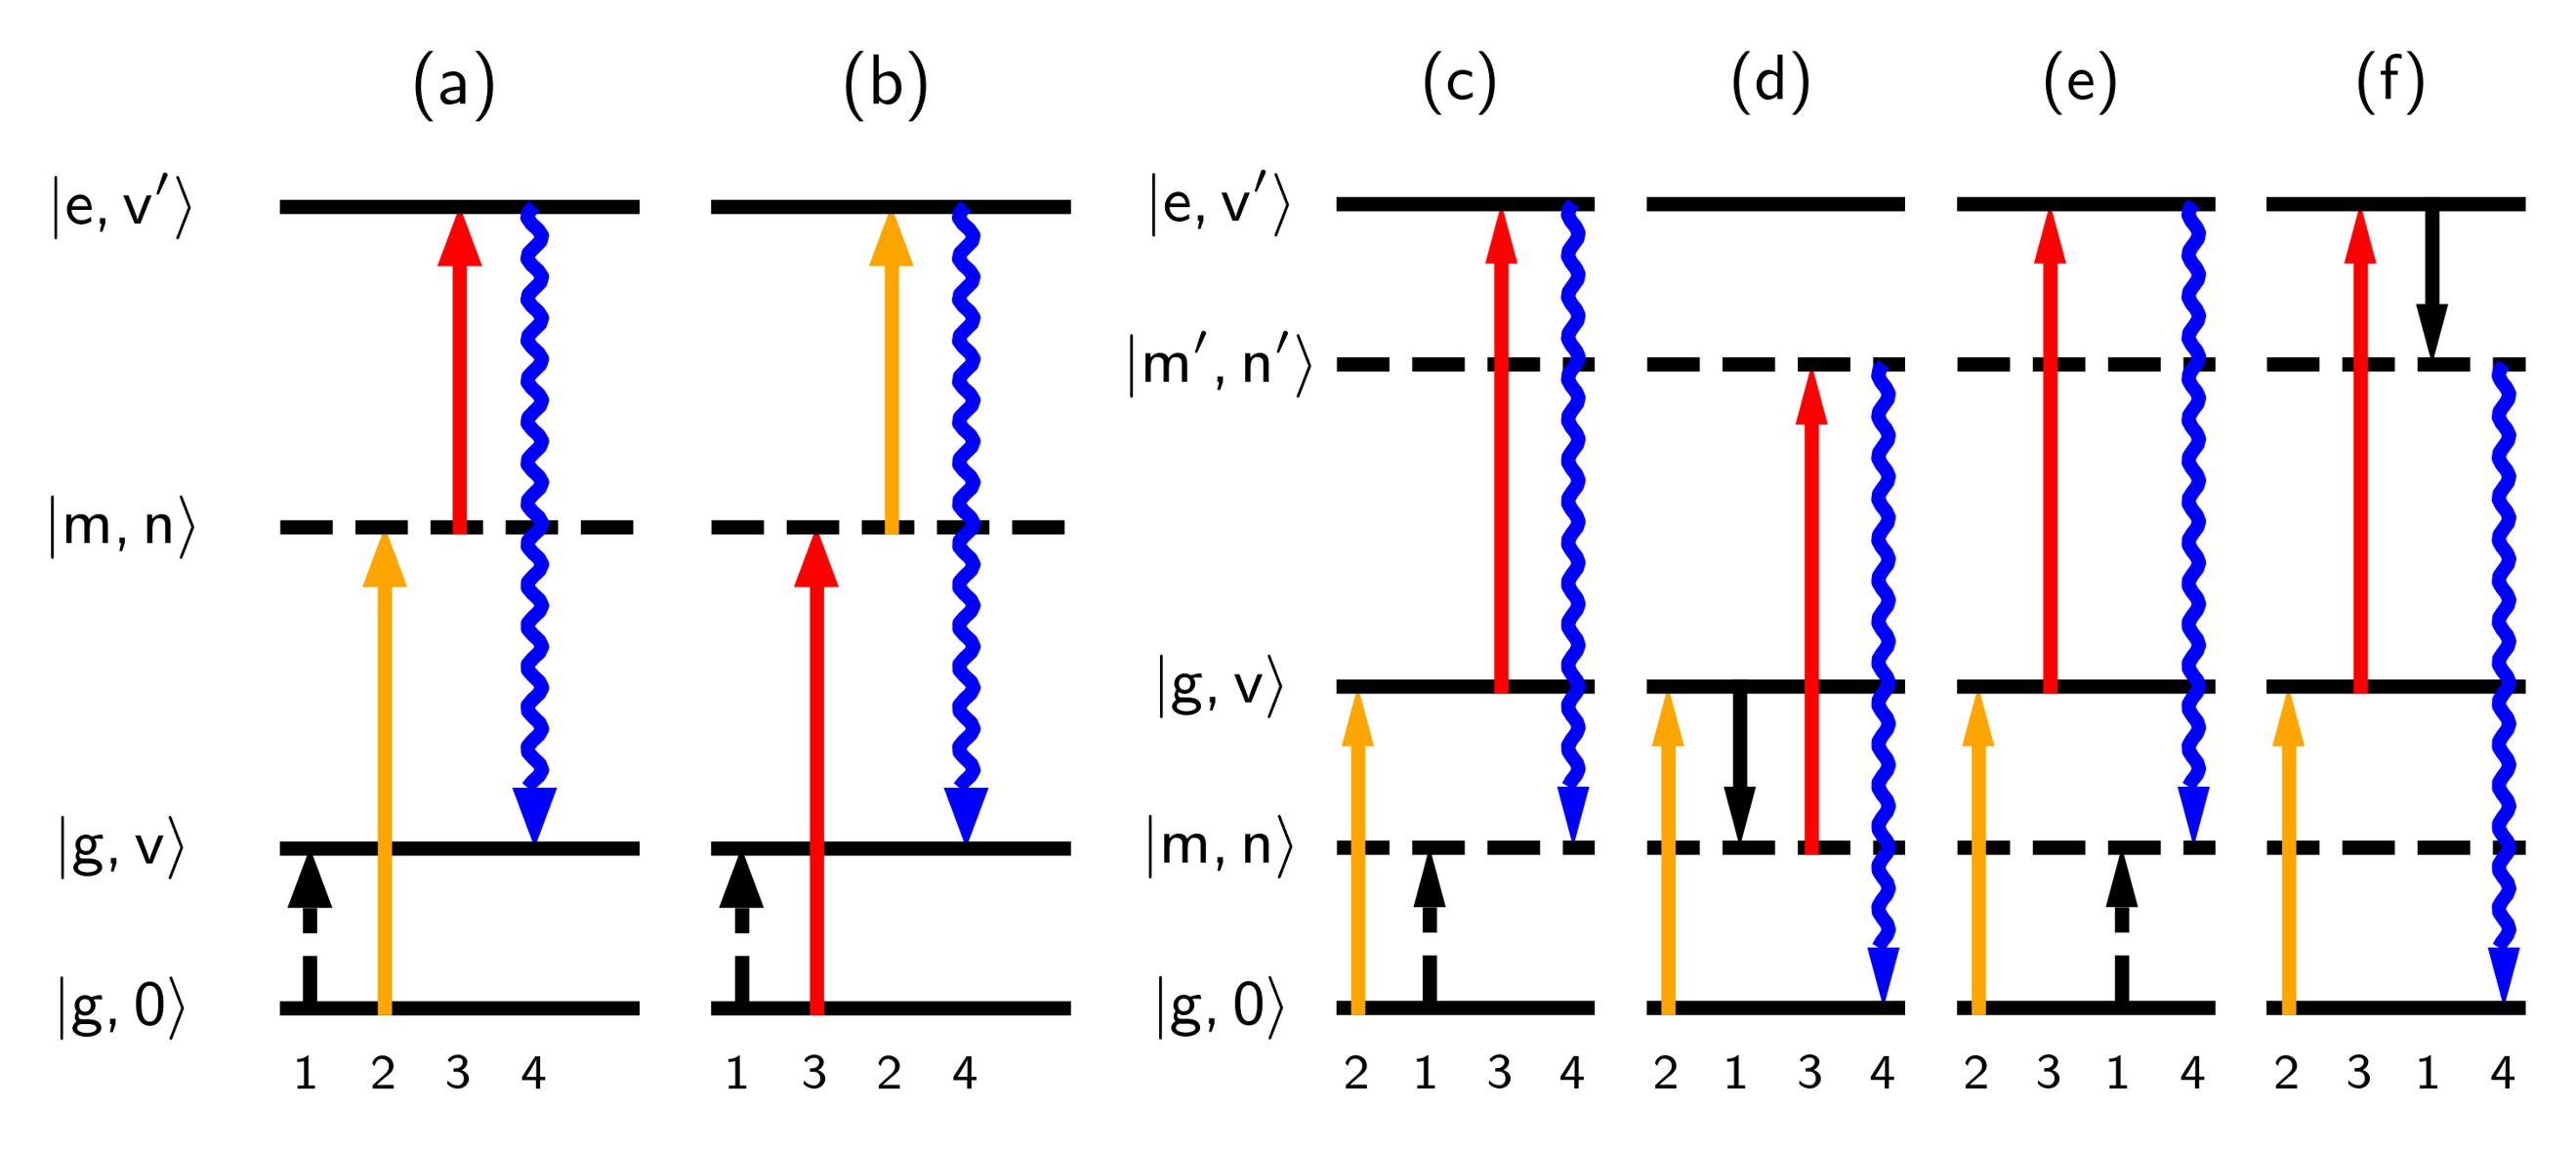
\includegraphics[width=6.66 in]{figures/timeorderedwmel.png}
	\caption{WMEL diagrams of HDFG pathways for when (a,b) $\omega_1$ (black arrow) interacts first and (c-f) $\omega_2$ (orange arrow) interacts first. 
		The states are labeled as $\ket{a,b}$, where $a$ refers to an electronic state and $b$ refers to quanta in a vibration on $a$, described in \autoref{Albrecht}.
		In all cases, $\omega_2 > \omega_1$.
	}
	\label{fig:sivewmel2}
\end{figure*}

In the limit where $\omega_2+\omega_3$ is detuned from an electronic resonance, it becomes simple to interpret the interference schemes. 
The case where $\omega_1$ interacts first and is resonant, and $\omega_2 + \omega_3$ is nonresonant, yields two contributed pathways: \autoref{fig:sivewmel2} (a) and (b).
These pathways possess identical phase and transition moments, which yields total constructive interference, assuming similar non-resonant dispersion from each pathway.
Conversely, in the case where only $\omega_2$ is vibrationally resonant, diagrams (c,d) and (e,f), when detuned from an electronic resonance, have identical transition moments but opposite phase. 
As a result, the output from (c,d) and (e,f) completely destructively interfere; no signal can be obtained from these pathways when significantly detuned. \cite{RN287, McDonnell2024}
Note that in the case where $\omega_1$ interacts first but $\omega_2$ is resonant, the nonlinear output generated nearly vanishes as the first resonant pulse arrives after a non-resonant pulse.

When $\omega_2 + \omega_3$ becomes electronically resonant, the interference changes for the \autoref{fig:sivewmel2}c-f pathways.
Note that in this regime, only pathways (c,e,f) possess identical transition moments.
As a result, pathways (c,d) survive and can provide output when $\omega_2+\omega_3$ is resonant with an electronic state. 
These results provide a simple rule of thumb for collecting HDFG spectra: use \autoref{fig:sivewmel2}a,b pathways to measure spectra when significantly detuned from an electronic resonance, and any of these vibrationally resonant pathway can measure spectra when electronically resonant.
However, since electronic states commonly have short dephasing times and significant inhomogeneous broadening,\cite{Dong2015, Lewis2015} it is likely the \autoref{fig:sivewmel2}f pathway will become triply resonant and possibly contribute greater than the other pathways. 
Such instances are system dependent. 
Discussion will be isolated to the \autoref{fig:sivewmel2}a pathway in the sections that follow.

Another potential interferant in HDFG spectroscopy is direct and sequential cascades of second-order vDFG and vSFG processes.\cite{RN297, RN301}
While unimportant in achiral isotropic systems,\cite{Belkin2000} second-order cascades may become important in media where SFG and DFG are allowed, e.g. chiral media, interfaces or non-centrosymmetric media. 
Nevertheless, in the discussion that follows for the rest of this manuscript, we will assume negligible second-order cascades. 

\subsection{Lineshape Models for HDFG Spectroscopy}


It is useful to expose relationships between nonlinear output, transition dipoles and hyper-Raman hyperpolarizabilities in the driven limit. \cite{Simpson2004}
Under the electric dipole approximation, the $I^\text{th}$ cartesian component of the third order nonlinear output polarization, ${P}^{(3)}_I$, of a four wave mixing process, induced by electric fields $E_J$, $E_K$, and $E_L$ at output frequency $\omega_4=-\omega_1 + \omega_2 + \omega_3$ is written as (using Einstein summation) \cite{RN307}
\begin{equation} \label{polarization}
{P}^{(3)}_I (\omega_4)  = \chi^{(3)}_{IJKL} E_J(\omega_3) E_K(\omega_2) E_L(\omega_1) 
\end{equation}
where $\chi^{(3)}_{IJKL}$ is the $IJKL$ element of the third order electrical susceptibility, a rank four tensor, generally written as
\begin{equation}\label{eq:nfgamma}
	\chi^{(3)}_{IJKL} = NF \langle \gamma_{ijkl} \rangle.
\end{equation}
Here $N$ is a number density and $\gamma_{ijkl}$ is the third-order polarizability (i.e., second hyperpolarizability).
The brackets indicate an orientational average.\cite{Andrews1977}
Uppercase letters refer to laboratory frame coordinates and lower case letters refer to corresponding molecular frame coordinates.
$F=\prod_j  \frac{1}{3} \left({\left(n(\omega_j)\right)^2 + 1} \right)$ is the Lorentz local field factor, where $n$ is the (frequency dependent) refractive index. \cite{Bedeaux1973}

By propagating density matrix elements in the steady state limit, the HDFG hyperpolarizability is \cite{RN133}
\begin{equation}\label{sivegamma}
		\gamma_{ijkl}^{vg} =	- \sum_{e,m} \frac{1}{\varepsilon_0} \frac{1}{4D} \frac{1}{\hbar^3} \frac{\mu^{ve}_{i} \mu^{em}_{j} \mu^{mg}_{k} \mu^{gv}_{l} }{\Delta_{ev}^{3+2-1} \Delta_{mv}^{2-1}\Delta_{gv}^{-1}}  \rho_{gg}
\end{equation}
where: $\mu^{ab}_{j}$ is the $j^{th}$ element of $\mel{a}{\vec{\mu}}{b}$, $\Delta_{kl}^{-x+y+z} = \omega_{kl} - (-\omega_{x}+\omega_{y} + \omega_{z}) - i\Gamma_{kl}$, $\omega_j$ is the frequency of the j$^{th}$ input field, $\Gamma_{kl}$ is the dephasing of $\rho_{kl}$ and $\rho_{gg}$ is the ground state population.
Here, $\ket{e}$ and $\ket{m}$ are virtual states, and thus necessarily summed over in \autoref{sivegamma}.
The pulse identifiers on the $\Delta_{kl}$ terms will be suppressed henceforth for simplicity.
$D$, the Maker-Terhune degeneracy factor, accounts for permutation symmetry of the excitation fields.\cite{RN134} 
For a HDFG experiment using two (three) distinct, non-degenerate input fields, $D = 3 (6)$.

\subsection{Vibrational Selection Rules}

It is useful to investigate the selection rules without vibronic resonance to understand how HDFG can be used as an upconverted infrared spectroscopy.
We first investigate the HDFG selection rules through a Placzek type formalism.
When $\omega_2+\omega_3$ is significantly detuned from resonance and the vibronic nature of the virtual states is ignored, the Placzek approximation can be used to study selection rules in terms of the hyper-Raman hyperpolarizability, $\beta$. \cite{Placzek1934, Long1970, Altmann1982}
Summing over the virtual states $\ket{e}$ and $\ket{m}$ forms the hyper-Raman hyperpolarizability so that\cite{Long1970} 
\begin{equation}\label{sivebeta}
	\gamma_{ijkl} =	-\frac{1}{\varepsilon_0} \frac{1}{4D \hbar}\frac{\beta^{vg}_{ijk} \mu^{gv}_{l}}{\Delta_{gv}} \rho_{gg}.
\end{equation}
Since all infrared active transitions are hyper-Raman active, HDFG is allowed for any infrared active transition. \cite{Andrews1978}
This selection rule is generally valid for any HDFG or HSFG process when $\omega_2$ and $\omega_3$ are sufficiently detuned from any resonance.

The general selection rule can be simplified by considering excitation of an infrared active normal mode.  
Assume state $v$ is the $v^{\text{th}}$ normal mode.
We Taylor expand the dipole and first hyperpolarizability operators to first order in the normal mode coordinate $Q_v$ about equilibrium:\cite{Long1970, Shen90}
\begin{subequations}
	\begin{equation}
		\mu_l = \mu_{l,0} + \left(\frac{\partial \mu_l}{\partial Q_v}\right)_0 Q_v 
	\end{equation}
	\begin{equation}
		\beta_{ijk} = \beta_{ijk,0} + \left(\frac{\partial \beta_{ijk}}{\partial Q_v}\right)_0 Q_v
	\end{equation}
\end{subequations}
Substituting into \autoref{sivebeta} gives the HDFG hyperpolarizability to $\order{Q_n}$ as \begin{equation}\label{SIVEselection}
	\gamma_{ijkl} =	-\frac{1}{\varepsilon_0} \frac{1}{8D \omega_{vg}}  \frac{1}{{\Delta_{gv}}} \ \left(\frac{\partial \beta^{vg}_{ijk}}{\partial Q_v}\right)_0 \left({\frac{\partial \mu^{gv}_{l}}{\partial Q_v}}\right)_0  \rho_{gg}
\end{equation}
where we have used $\mel{1}{\mu_{l,0}}{0} = 0 = \mel{1}{\beta_{ijk,0}}{0}$, and $\mel{v}{Q_v}{g} \equiv \mel{1}{Q_v}{0} = \sqrt{\frac{\hbar}{2\omega_{vg}}}$. Here, $\omega_{vg}$ is the characteristic $\ket{0} \rightarrow \ket{1}$ frequency.\cite{RN459}
Since \autoref{SIVEselection} is non-zero in the harmonic oscillator limit, HDFG output is allowed for infrared active normal modes in the harmonic limit. 

\subsection{Vibronic Selection Rules}\label{Albrecht}
While the Placzek treatment provides the general source of HDFG output, it does not predict the behavior of $\beta_{ijk}$ as $\omega_2 + \omega_3$ is changed.
We now explicitly consider electronic resonances through the $A,B,C$ decomposition of $\beta$ introduced by Chung and Ziegler, analogous to those found in Albrecht's treatment of Raman spectroscopy.\cite{Albrecht1961, Ziegler1988} 
To employ this formalism, we write the states in a Born-Oppenheimer basis $\ket{a,b}$, where $\ket{a,b} = |a(Q)) \otimes \ket{b}$ for electronic states $\{|a(\textbf{Q}))\}$ and vibrational states $\{\ket{b}\}$ (i.e., adiabatic approximation), where \textbf{Q}, the system normal modes, is the adiabatic parameter. \cite{BornOppenheimer, Tang1970}
We will henceforth suppress the dependence of the electronic states on \textbf{Q} for simplicity.

For consistency with previous reports, we use $\vec{R}$ to denote electric transition dipole moments; $\vec{\mu}$ is reserved for transitions on the ground electronic state. \cite{Tang1970}
Following the approach which gave \autoref{sivegamma} and using the time ordering and state labeling of \autoref{fig:sivewmel2}a, we find
\begin{equation}\label{drgamma_notaylor}
	\gamma_{ijkl} = -\frac{1}{\varepsilon_0} \frac{1}{4D \hbar^3} \sum_{m,n,e,v'} \frac{
		R_{i}^{gv, ev'} 
		R_{j}^{ev',mn} 
		R_{k}^{mn,g0} 
		R_{l}^{g0,gv} 
	}{	\Delta_{ev', gv}
		\Delta_{mn, gv}
		\Delta_{g0,gv}
	}
\end{equation}
where $R_{i}^{ab,cd}$ is the i$^{th}$ element of $\mel{a,b}{\vec{R}}{c,d}$.
It is common in the hyper-Raman literature to write $\Delta_{ev', gv} \Delta_{mn, gv} = \Delta_{ev', gv}$.
Using our definition of vibronic states, we can write, for example,
$R_{i}^{gv,ev'} = \mel{v}{M_i^{ge}}{v'}$, where $\vec{M}^{ab} = (a|\vec{R}|b)$.\cite{Ziegler1974}
Expanding $\vec{M}^{ij}$ to $\order{Q}$ about the equilibrium point of the ground state potential surface as
$\vec{M}^{ij} = \vec{M}^{ij}_0 + \sum_z \frac{\partial\vec{M}^{ij}}{\partial Q_z} Q_z$
yields $A, B, C$ coefficients similar to those in the Albrecht formalism of Raman scattering, \cite{Albrecht1961, Warshel1977, Ziegler1988} so that
\begin{equation}\label{gammaabc}
		\gamma_{ijkl} \sim \left(A_{ijk} + B_{ijk} + C_{ijk}\right) \frac{\mel{v}{\mu_{l}}{0}} {\Delta_{g0,gv}}
\end{equation}
The $A$ term contains the static ($\order{Q^0}$) transitions (i.e., Condon approximation), the $B$ term depends upon $\order{Q}$ transitions (Herzberg-Teller contributions), and the $C$ term depends on $\order{Q_i Q_j}$ transitions. 
The $C$ term is suppressed in the following discussion as it depends on one and two photon forbidden transitions, making its contribution to $\gamma_{ijkl}$ roughly two orders of magnitude less than $A_{ijk}$. \cite{Ziegler1988, Neddersen1989, Bonang1992}
Note that some reports obtain $A, B$ coefficients through a Herzberg-Teller expansion of the electronic states to expose vibronic couplings via $\partial H / \partial Q$, where $H$ is the electronic Hamiltonian.\cite{HerzbergTeller1933, Petrov1985, Neddersen1989, Baranov1990}
This approach is not used here as the expansion of $\vec{M}^{ij}$ in normal mode coordinates provides sufficient physical insight into hyper-Raman selection rules. 

The $A$ and $B$ coefficients, where $B = B_1 + B_2$, following closure over $\ket{n}$,\cite{Milojevich2013} are written as:
\begin{widetext}
\begin{subequations}\label{ABterms}
\begin{equation}
	\begin{split}
		A_{ijk} = \frac{1}{\hbar^2}\sum_{m,e,v'} M^{ge}_{0,i} 
		M^{em}_{0,j} 
		M^{mg}_{0,k}
		 \langle v | v' \rangle
		 \langle v' | 0 \rangle 
		 \frac{1}{\Delta_{ev', gv}}
		 \\
	\end{split}
\end{equation}
	\begin{equation}
		\begin{split}
			B_{1_{ijk}} &= \frac{1}{\hbar^2} \sum_{m,e,v',z} M^{ge}_{0,i} \left(
				\frac{\partial M^{em}_{j}}{\partial Q_z} M^{mg}_{0,k}  
				+M^{em}_{0,j} \frac{\partial M^{mg}_{k}}{\partial Q_z}
			\right)
			\langle v | v' \rangle \mel{v'}{Q_z}{0} \frac{1}{\Delta_{ev', gv}}\\
		\end{split}
	\end{equation}
	\begin{equation}
	\begin{split}
			B_{2_{ijk}} = \frac{1}{\hbar^2} \sum_{m,e,v',z} \frac{\partial M^{ge}_{i}}{\partial Q_z} M^{em}_{0,j} 
			M^{mg}_{0,k} \mel{v}{Q_z}{v'} 
			\langle v' | 0 \rangle 
			\frac{1}{\Delta_{ev', gv}}
	\end{split}
	\end{equation}
\end{subequations}
\end{widetext}
where $\langle a | b \rangle$ and $\mel{a}{Q}{b}$ are Franck-Condon factors and Herzberg-Teller-type integrals, respectively. 
Duschinsky rotation effects are ignored in this discussion. \cite{Duschinsky1937}
At this point, the expressions are valid for both electronically resonant and non-resonant cases.

To understand the vibronic structure of electronic resonance, we restrict consideration to electronic transitions between $|g)$ and $|e)$.  
Note that HDFG experiments selectively excite ground state vibrational modes through $\omega_1$; we will assume the IR beam has excited the fundamental of an IR-active mode so that hyper-Raman scattering is between this mode and the ground state. 
By working only in terms of this single normal mode (i.e., removing the sum over $z$ and taking $v=1$), 
the $A$ and $B$ terms are rewritten as 
	\begin{subequations}\label{ABterms_DR}
		\begin{equation}
			\begin{split}
				A_{ijk} = \frac{1}{\hbar}\sum_{v'} M^{ge}_{0,i} 
				\Lambda^{eg}_{0,jk}
				\langle 1 | v' \rangle
				\langle v' | 0 \rangle 
				\frac{1}{\Delta_{ev',gv}}
				\\
			\end{split}
		\end{equation}
		\begin{equation}
			\begin{split}
				B_{1_{ijk}} &= \frac{1}{\hbar} \sum_{v'} M^{ge}_{0,i}
				\frac{\partial \Lambda^{eg}_{jk}}{\partial Q} \langle 1 | v' \rangle \mel{v'}{Q}{0} 
				\frac{1}{\Delta_{ev', gv}}\\
			\end{split}
		\end{equation}
		\begin{equation}
			\begin{split}
				B_{2_{ijk}} = \frac{1}{\hbar} \sum_{v'} \frac{\partial M^{ge}_{i}}{\partial Q} 
				\Lambda^{eg}_{0,jk} 
				\mel{1}{Q}{v'} 
				\langle v' | 0 \rangle 
				\frac{1}{\Delta_{ev',gv}}
			\end{split}
		\end{equation}
	\end{subequations}
where $\Lambda^{ab}_{ij} = 1/\hbar \sum_m M_i^{am}M_j^{mb} $ is the electronic two photon transition moment between $a$ and $b$.\cite{McClain1977}

\begin{figure*}[!htbp]
	\centering
	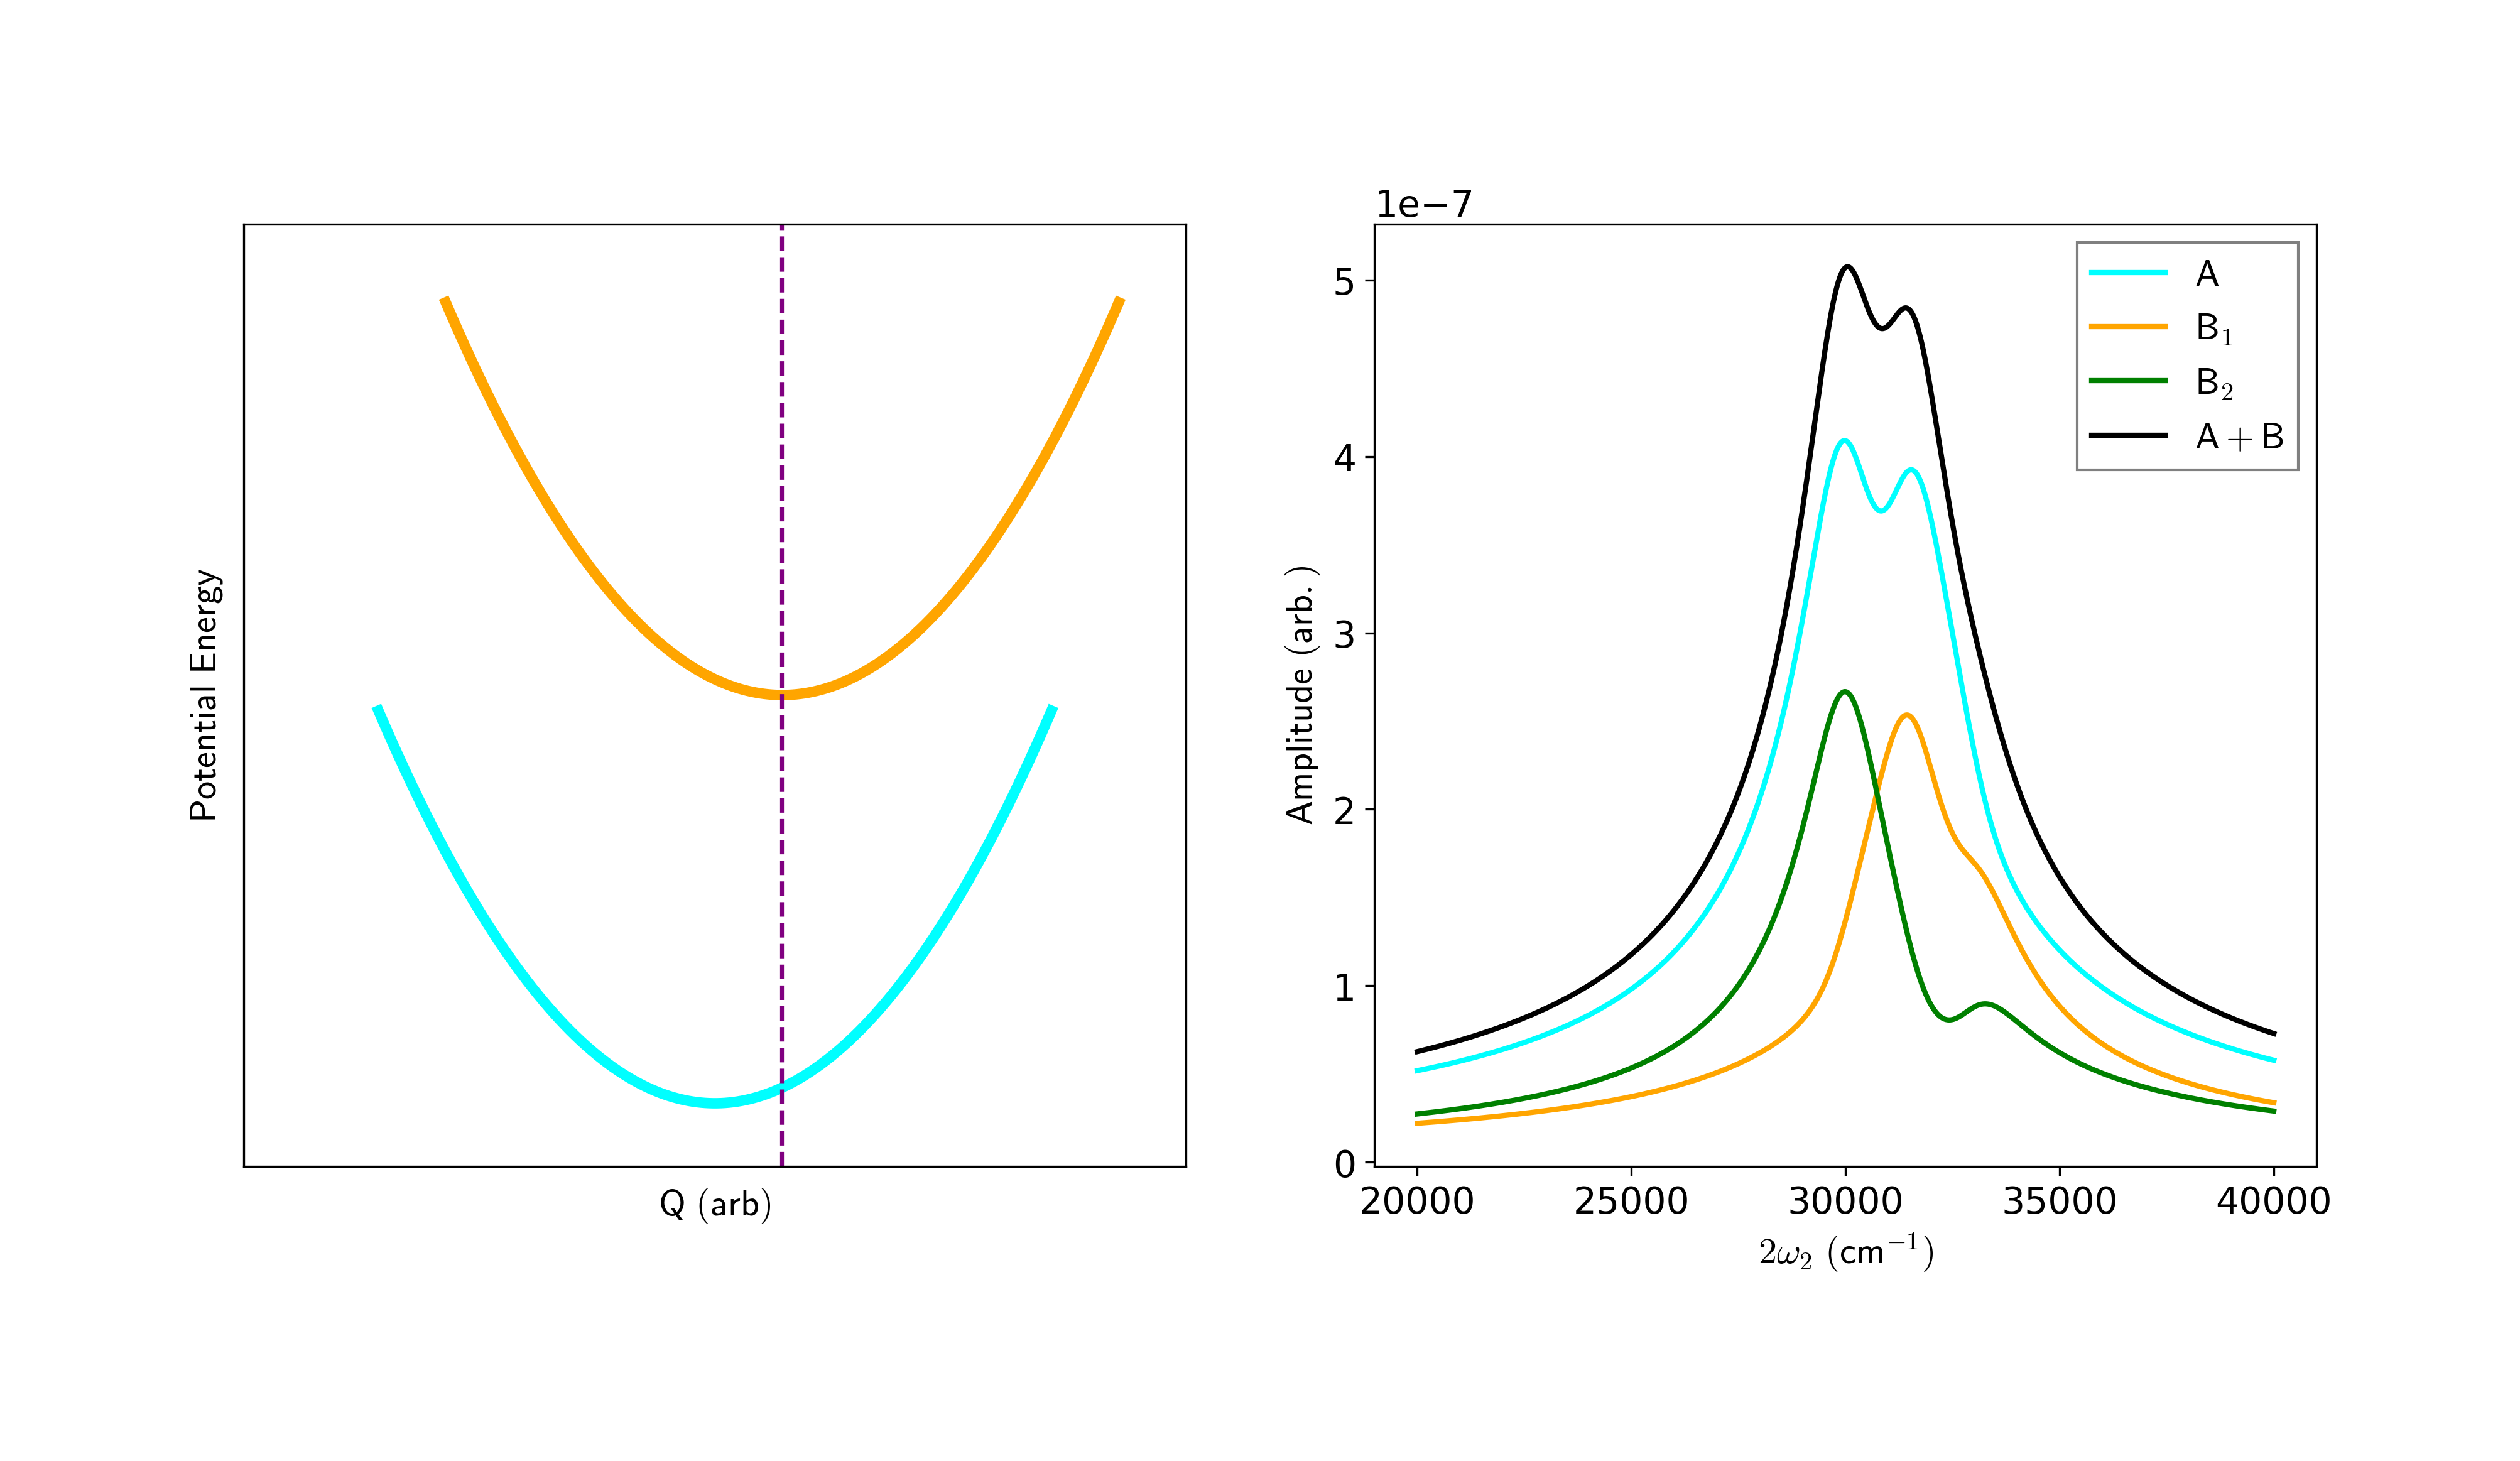
\includegraphics[width=6.66in]{drsive_spectrum.png}
	\caption{Contributions of $A, B$ (\autoref{ABterms_DR}) to HDFG spectrum for a simple two harmonic well system.
		(a) Potential energy surfaces for a two-well system, (b) 1D HDFG spectrum for $\xi = 0.5$, $\omega_1 = \omega_{g1, g0}$. 
		It is assumed that $\omega_2 = \omega_3$.
		Note that (b) plots magnitudes of the labeled quantities.
		The vibrational states on the $|g)$ and $|e)$ manifolds are spaced 2200 cm$^{-1}$ apart, with the vibronic states $\ket{e,v'}$ given linewidths of 700 cm$^{-1}$ and $\hbar \omega_{eg}$ = 30000 cm$^{-1}$.
		Dotted lines in (b) denote the $v'$ = 0, 1, 2 vibronic resonances. 
		The vibronic one and two photon absorption operators are scaled such that $\abs{B}/\abs{A} \sim$ 0.1, following Chung and Ziegler. \cite{Ziegler1988}
		The Franck-Condon and Herzberg-Teller contributions to each of these terms are found in \autoref{T:contributions}.}
	\label{fig:doubres_spec}
\end{figure*}

The signatures of vibronic coupling in the HDFG spectrum are made clear by using a simple model.
Using a two-well system described by $H = H_g |g) \left(g| + H_e |e\right) (e|$ where
\begin{subequations}\label{Hamiltonian}
	\begin{equation}
		H_g = \frac{\hbar \omega }{2} \left(p^2 + q^2 \right)
	\end{equation}
	and
	\begin{equation}
		H_e = \frac{\hbar \omega }{2} \left(p^2 +  (q-\xi)^2 \right) + \hbar \omega_{eg}
	\end{equation}
\end{subequations}
for the ground ($H_g$) and first excited ($H_e$) states, where $p$ (momentum) and $q$ (position) are the dimensionless conjugate coordinates of the normal mode, the A and B contributions can be evaluated using Franck-Condon and Herzberg-Teller integrals tabulated in terms of the dimensionless normal mode $q$ and offset parameter $\xi$ (\autoref{fig:doubres_spec}a).\cite{Carlson1988thesis} 
For simplicity, we restrict consideration to $v^\prime \in \{0,1,2\}$ and take $\xi = 0.5$.
Note that $q = \sqrt{\frac{m^2\omega}{\hbar}} Q$.
We assume the electronic state is both one and two photon allowed.

\autoref{ABterms_DR} shows important selection rules for the vibronic transitions.
The $A$ term is allowed whenever an electronic transition has a one- and two- photon transition moment.
For centrosymmetric molecules, an electronic transition cannot be both one- and two- photon allowed by parity, so the $A$ term will vanish.
This makes HDFG a unique tool for studying the electronic structure of centrosymmetric species in isotropic media, as it is sensitive to non-Condon effects.\cite{Olson2018}
For an allowed electronic transition, the brightness of a vibronic resonance is controlled by overlap of ground and excited state vibrational wavefunctions (Franck-Condon factors).
The $A$ term relies on excited state perturbations to the vibrational wavefunctions; if the excited electronic state minimally changes potential energy surface, so that ground and excited state vibrational eigenfunctions are identical, $\langle 1 | v^\prime \rangle \langle v^\prime | 0 \rangle = 0$ and $A$ vanishes.
This follows from $\lim_{\xi \rightarrow 0} \langle v' | 0 \rangle = 0$, $v^\prime \neq 0$, for wells with identical curvature.
Some $B$ terms do survive in the same limit, however; for instance, $B_1$ survives for $v^\prime=1$ and $B_2$ survives for $v^\prime=0$.
In the absence of an $A$ term, the $B$ terms will dominate.
The $B_1$ and $B_2$ terms involve different types of vibronic coupling pathways.
In $B_1$, the Herzberg-Teller coupling is associated with the two-photon absorption process, whereas in $B_2$, the Herzberg-Teller coupling is associated with one-photon emission.

\autoref{fig:doubres_spec}b shows the simulated $\omega_2+\omega_3$ spectrum for this two-well system.  The spectrum selectively probes vibronic pathways from $\ket{g,0}$ to $\ket{g,1}$.
In the resonant region, the $A$ and $B$ terms contain character from all three possible transitions between $\ket{g,0}$, $\ket{e,v'}$ and $\ket{g,1}$. 
Significant contributions from $\ket{e,0}$ and $\ket{e,1}$ in the $A$ term spectrum correspond well with expectations given the relative wavefunction overlap in \autoref{fig:doubres_spec}a, tabulated in \autoref{T:contributions}. 
Similarly, the $B_1$ term is dominated by coupling with the $\ket{e,1}$ state and $B_2$ is dominated by coupling with the $\ket{e,0}$ state (\autoref{T:contributions}). 
Note that contributions involving $\ket{e,2}$ are suppressed relative to the $\ket{e,0}$ and $\ket{e,1}$ contributions in the $A$ and $B$ terms.
This is expected, considering the large change in quantum number when involving $\ket{e,2}$ and the offset of the potential wells in \autoref{Hamiltonian}.

In the pre-resonance region, both $A$ and $B$ terms die off as $\sim \Delta_{e0,gv}^{-1}$.
We point this out because a persistent belief in Raman analysis is that $A$ terms disappear and $B$ terms dominate when significantly detuned from electronic resonance.
% such that $\Delta_{ev', g0} \approx \Delta_{eg}$, i.e., the resonance denominator loses $\ket{v'}$ dependence. 
The belief arises from the approximation $\abs{\omega_{ev',gv} - 2\omega_2} \gg 2\Gamma_{ev',gv}$, which then removes $A$ through a closure relationship.\cite{Neddersen1989}
As has been discussed elsewhere, however, this approximation is in many cases invalid, especially when vibrational energies are large, like those explored here.\cite{Warshel1977, Li1990, Gong2015}
This means that it is difficult to isolate $B$ terms when $A$ terms are present.
As such, HDFG will have difficulty examining non-Condon effects ($B$ term contributions) noncentrosymmetric systems.

\begin{table}[!htbp]
	\caption{\label{T:contributions} Franck-Condon and/or Herzberg-Teller contributions to $A$, $B_1$, $B_2$ terms between $\ket{g,0}$, $\ket{g,1}$ and vibronic states $\ket{e,0}$, $\ket{e,1}$, $\ket{e,2}$ for \autoref{Hamiltonian} with an offset $\xi = 0.5$.
	Closed-form expressions for the Franck-Condon and Herzberg-Teller integrals used here have been tabulated by Carlson.\cite{Carlson1988thesis}}
	\begin{ruledtabular}
		\begin{tabular}{cccc}
			$2\omega_2$ Electronic Resonance & $\ket{e,0}$ & $\ket{e,1}$ & $\ket{e,2}$\\
			\hline  
			$A$ 
			& $\langle 1 | 0 \rangle \langle 0 | 0 \rangle = 0.31 $  
			& $\langle 1 | 1 \rangle \langle 1 | 0 \rangle = 0.27 $ 
			& $\langle 1 | 2 \rangle \langle 2 | 0 \rangle = -0.04$\\
					
			$B_1$ 
			& $\langle 1 | 0 \rangle \mel{0}{Q}{0} = -0.08$ 
			& $\langle 1 | 1 \rangle \mel{1}{Q}{0} = 0.48$ 
			&$\langle 1 | 2 \rangle \mel{2}{Q}{0} = 0.14$\\
						
			$B_2$ 
			& $\mel{1}{Q}{0} \langle 0 | 0 \rangle = 0.55$  
			& $\mel{1}{Q}{1} \langle 1 | 0 \rangle = -0.07$ 
			& $\mel{1}{Q}{2} \langle 2 | 0 \rangle = 0.08$\\
		\end{tabular}
	\end{ruledtabular}
\end{table}

\subsection{Line Narrowing in SIVE Spectroscopies}
An unavoidable consequence in electronic spectroscopy is broadened lineshapes due to the inhomogeneity of electronic transitions (e.g., vibronic sidebands, molecular collisions). 
Four wave mixing methods can line-narrow transitions and remove some impact of inhomogeneous broadening.\cite{Carlson1990line}
The line-narrowing properties of DR-SIVE are investigated so that the pathways which line-narrow correlated or anti-correlated modes (\textit{vide infra}) can be identified.
SR-SIVE cannot linenarrow transitions as it is singly resonant. \cite{RN352}
In the discussion that follows, we assume that a vibrational mode in the ground state, $\ket{g,v}$, is correlated to the frequency of a vibronic $\ket{e,v'}$.\cite{Carlson1990line, Dong2015}
If the frequency of $\ket{g,v}$ is written as $\omega_{gv} + \xi$, where $\xi$ is some external strain (e.g. molecular collisions), then the frequency of $\ket{e,v}$ is $\omega_{ev} + c\xi$, where c is a shift coefficient.
Similarly, we take the frequency of $\ket{e,0}$ as $\omega_{e0} \rightarrow \omega_{e0} + \xi$.
The strains shift resonance denominators, e.g., for $\omega_{ij} \rightarrow \omega_{ij} + c\xi$, as
\begin{equation}
	\Delta_{ij}(\xi) = \omega_{ij} + c\xi -\omega_k - i\Gamma_{ij} \equiv \Delta_{ij}(0) + c\xi
\end{equation}
Without loss of generality, we assume c = 1 for correlated modes and c = -1 for anti-correlated modes.
To understand the impact of inhomogeneity on spectral output, we convolute an output density matrix element $\rho_{ab}(\xi)$ with a normalized Lorentzian distribution $P(\xi)$ of half width $\sigma$ as \cite{Penner1976, Desiderio1979, Dick83_1, Carlson1990line} 
\begin{equation}\label{contour}
	\rho_{ab} = \int_{-\infty}^\infty \mathrm{d}\xi P(\xi) \rho_{ab}(\xi)
\end{equation} 
While Gaussian distributions are commonly used to describe inhomogeneous broadening,\cite{RN307} Lorentzian distributions have successfully described inhomogeneous broadening in a variety of spectroscopies and yield easily interpreted closed-form solutions. \cite{Dick83_1, Carlson1990line}

By substituting the output density matrix elements for HSFG and non-parametric HDFG into \autoref{contour}, it is clear that HSFG line-narrows anti-correlated modes, whereas non-parametric HDFG line-narrows correlated modes. 
See the supporting information for more information.
Although \autoref{contour} identifies that only nonparametric HDFG line-narrows correlated modes, these results are only valid in limits where the input pulses only weakly populate excited states.
When resonant pulses are significantly longer than the dephasing time of some state, then that state can become populated.
Excited state population effects are particularly important for understanding the spectroscopy of electronic states using input pulses with pulsewidths significantly longer than dephasing times. \cite{RN319, Yurs2012}
Excited state populations can feed other modes, including the ground state and other vibrational/vibronic modes, inducing higher order processes.\cite{Carlson87, RN471}
These feeding mechanisms can induce line-narrowing properties in spectroscopies that cannot line-narrow in third order perturbation theory.\cite{RN319, Carlson87, RN471, RN410}

\section{Quantitative Aspects of HDFG}\label{quant}
% Despite their increasing use for dissecting intra and intermolecular interactions, CMDS techniques are usually not feasible for most laboratories, as they usually demand the use of multiple optical parametric amplifiers and/or complex acousto-optic modulators. \cite{Chen2016}
% Unlike most four wave mixing techniques, HDFG can be performed using only two input beams (i.e., two color HDFG).
% 


\subsection{vSFG detection levels are adequate for HDFG}

Can vSFG experimental setups detect HDFG signals?
SFG setups typically leverage the surface selectivity of $\chi^{(2)}$ polarizations,\cite{RN132, RN133} which results in extremely small emission volumes, so SFG setups are typically quite sensitive.
However, HDFG is a weak $\chi^{(3)}$ process because it depends upon hyper-Raman cross-sections, which are commonly several orders of magnitude weaker than corresponding Raman transitions.\cite{RN515}
Since HDFG can be performed as a two-beam experiment, it is useful to identify whether vSFG and HDFG responses are similar to quantify hyper-Raman-based FWM response from bulk, isotropic systems.
To evaluate the feasibility of HDFG for vSFG practitioners, we have compared the relative output of each process using nominal parameters. 
As calculated in \autoref{appendixA}, HDFG's weak $\chi^{(3)}$ value and SFG's low emission cancel somewhat, so that the output polarization of HDFG and vSFG are comparable ($\abs{P_\text{vSFG} / P_\text{HDFG}} \sim 1$).
Transient HDFG, or IR-pump-HDFG-probe, analogous to IR-pump-vSFG-probe, is therefore also feasible under similar experimental conditions, and provides vSFG practitioners a simple method to measure bulk dynamics without significant changes in an experimental setup. 
Therefore, HDFG is a feasible spectroscopy for practitioners of vSFG both in terms of experimental setup and detection feasibility.


\subsection{Extraction of hyper-Raman hyperpolarizability}

Compared to $\vec{\mu}$ and $\alpha_{ij}$, it is difficult to measure $\beta_{ijk}$ values through spontaneous hyper-Raman experiments.\cite{Kelley2010}
Only a few experimental determinations of $\beta_{ijk}$ for vibrational modes have been performed.\cite{Xu1997, Shoute2005, Kelley2010}
Methods reported in the literature to measure absolute hyper-Raman polarizabilities depend upon internal standards such as hyperpolarizabilities of dissolved samples or two-photon absorption cross sections, also difficult to measure. \cite{Kelley2010} 
In the method introduced by Levenson and Bloembergen (Bloembergen interferometry experiment), an internal standard interferes with the resonant lineshape of a $\chi^{(3)}$ process. \cite{Levenson1974_1, Levenson1974_2}
Self-heterodyning of the internal standard signal measures $\chi^{(3)}$ and does not require measurement of absolute intensities. 
Since the Bloembergen interferometry experiment only relies on the third order susceptibility for measured species (e.g., benzene or CaF$_2$),\cite{Levenson1974_2} it is possible to use quantitative four wave mixing spectroscopy to calculate $\beta_{ijk}$ values for infrared active vibrations.
It is thus useful to investigate how a treatment of orientational averaging can extract $\beta_{ijk}$ from the HDFG $\chi^{(3)}_{IJKL}$ expression.

Using \autoref{eq:nfgamma} and \autoref{sivebeta}, we can write
\begin{equation}\label{chi3}
		\chi^{(3)}_{IJKL} = -\frac{NF}{4D \hbar \varepsilon_0 \Delta_{gv}} \langle \beta_{ijk} \mu_l \rangle \rho_{gg}\\
\end{equation}
For simplicity, we take $\rho_{gg} = 1$.
The steps behind orientational averaging of $\gamma_{ijkl}$, a rank four tensor in the molecular frame, are detailed elsewhere.\cite{Andrews1977, McDonnell2024}
Briefly, a tensor in the molecular frame, $A_{ijkl}$, is transformed into an element of the same tensor in the laboratory frame, $\langle A \rangle_{IJKL}$, through $\langle A \rangle_{IJKL}$ = $\theta^{ijkl}_{IJKL} A_{ijkl}$, where summation over repeated indices is implied and $\theta$ is the transformation operator. \cite{McDonnell2024, Andrews1977}
Orientational averaging shows specific polarization schemes isolate linear combinations of different $\beta_{ijk}$ terms. \cite{Bersohn1966, Willetts1992, Kauranen1996}
Substituting in \autoref{SIVEselection}, we see
\begin{equation}\label{betasive}
	\left\langle \frac{\partial \beta}{\partial Q_v} {\frac{\partial \mu}{\partial Q_v}} \right\rangle _{IJKL} = -\frac{8D \varepsilon_0}{NF}  {\Gamma_{gv} \omega_{vg}} \chi^{(3)}_{IJKL}
\end{equation}
$\chi^{(3)}$ itself can be extracted with use of an internal standard.\cite{Levenson1974_1, Levenson1974_2}
Since $\abs{\partial \mu / \partial Q}$ values can be extracted from FT-IR spectra,\cite{RN459} HDFG can give quantitative information on the magnitude of $\beta_{ijk}$ for infrared active vibrations.
Additionally, by using non-degenerate input frequencies to stimulate the hyper-Raman transition, the asymmetric properties of $\beta_{ijk}$ can be examined and quantified. \cite{Christie1971, Denisov1986, Kozich2007}
These quantitative aspects of HDFG could prove useful for examining how well computational methods calculate $\beta_{ijk}$ values.

\section{Conclusions}\label{conclusion}
Coherent vibrational, hyper-Raman coherent four wave mixing spectroscopies are identified and discussed.
Hyper difference frequency generation (HDFG) possesses infrared absorption and vibronic hyper-Raman scattering selection rules.
As a result, HDFG output is sensitive to the relative overlap of potential energy surfaces.
In HDFG, using the Chung-Ziegler approach to vibronic hyper-Raman scattering, output is dependent upon changes in different potential energy surfaces along the coordinate of the vibrational mode selected by the infrared input. 
If the potential energy surface is not significantly modulated along the vibrational coordinate of interest, then output is dominated by $B$ term resonances, i.e. Herzberg-Teller coupling.
As a result, HDFG possesses types of site-selective properties analogous to those of coherent Raman experiments, which can allow for a thorough analysis of vibronic coupling schemes in isotropic systems.
We show that HDFG provides alternative methods to extract the hyper-Raman hyperpolarizability of infrared active vibrations. 
Since HDFG is approachable as a two-beam experiment, analogous to vibrational sum-frequency generation, and phase-matchable in media with normal dispersion, HDFG should be applicable towards understanding vibrational spectroscopy and dynamics, e.g. single quantum coherence free induction decay dynamics, in a variety of relevant molecular and materials systems.  

\section{Data Availability Statement}
The workup scripts that support this study are permissively licensed and available for reuse at \href{https://osf.io/2amkq/}{https://osf.io/2amkq/}.

\section{Acknowledgments}
This work received support from the National Science Foundation (Grant no. CHE-2203290).
R.P.M. acknowledges support from the National Science Foundation Graduate Research Fellowship Program (Grant no. DGE-2137424). 

\section{Appendix: Comparison of vSFG and two-beam HDFG output}\label{appendixA}
To motivate the application of HDFG spectroscopy, we perform a calculation to compare two-color HDFG and vSFG output, where absorption effects are neglected for simplicity. \cite{Carlson1989}
vSFG is a $\chi^{(2)}$ technique, when only vibrationally resonant, whose output scales as $\chi^{(2)}_{IJK} \sim \langle \alpha_{ij} \mu_k \rangle$, where $\alpha_{ij}$ is the Raman polarizability tensor.
The output polarizations for vSFG and HDFG, respectively, under the electric dipole approximation are written as
	 	\begin{subequations}
		 	\begin{equation}\label{PSFG}
		 		\begin{split}
		 		\abs{P^{(2)}_{\text{vSFG}}} &= \frac{N_\text{surf}}{\ell} \abs{F_{\text{SFG}} \langle \alpha_{ij}\mu_{k} \rangle E(\omega_2)E(\omega_1)} 
		 		\end{split}
			 \end{equation}
		 	\begin{equation}
		 		\begin{split}
			 		\abs{P^{(3)}_{\text{HDFG}}} &= N_\text{bulk} \abs{F_{\text{HDFG}} \langle \beta_{ijk} \mu_{l} \rangle E{(\omega_2)}E(\omega_2)E(-\omega_1)}
		 		\end{split}
			 \end{equation}
		 \end{subequations}
where N$_\text{bulk}$ is the bulk number density ($\sim$ 10$^{28}$ m$^{-3}$ for H$_2$O$_{(l)}$ at room temperature), and N$_\text{surf}$ is the surface number density ($\sim$ 10$^{16}$ m$^{-2}$ for H$_2$O adsorbed at quartz).\cite{Du1994}	
For simplicity, we assume that $\chi^{(2)}$ is a spatial constant so that $\int_{0^-}^\ell \mathrm{d}z \langle \alpha_{ij}\mu_{k} \rangle \approx \ell \langle \alpha_{ij}\mu_{k} \rangle$, where $z$ is oriented along the surface normal and $0^{-}$ is the edge of the interface where substrate begins. 
We take the film thickness ($\ell$) probed by vSFG to be 1 nm, much less than the vSFG coherence length.\cite{RN133}
A normal dispersion curve is assumed so that $n(\omega_1+\omega_2) \approx n(2\omega_2-\omega_1)$.
To simplify analysis, orientational averaging is ignored (e.g., $\langle \beta_{ijk} \mu_{l} \rangle \approx \beta \mu$) and the input and output fields are taken to be co-polarized, so that
\begin{equation}
	P_\text{ratio} \equiv \frac{\abs{P^{(3)}_{\text{HDFG}}}}{\abs{P^{(2)}_{\text{vSFG}}}} \approx \frac{N_\text{bulk}}{N_\text{surf}} \abs{\frac{\left(n(\omega_2)\right)^2 + 1}{3}} \frac{\beta}{\alpha} E(\omega_2) \ell \sim 10^3 \frac{\beta}{\alpha} E(\omega_2)\\
\end{equation}
Ziegler has noted that for a field with intensity 10 GW/cm$^{2}$, $\frac{\beta E}{\alpha} \sim 10^{-3} $ for vibrational modes when detuned from electronic resonances, i.e. singly resonant vSFG and HDFG. \cite{RN515}
Such an intensity is easily obtained using modern ultrafast sources.
In this limit, $P_\text{ratio} \sim 1$, or the HDFG output is roughly as strong as vSFG, assuming only interfacial contributions in vSFG.
It is important to note that this calculation assumed negligible dipole and Raman polarizability dependence upon the distance from surface normal, ignored orientational averaging effects, and presumed equivalence of local field factors, all of which can significantly reduce output from either process. 
Nevertheless, since HDFG produces a similar number of photons as vSFG, HDFG is a viable technique for investigating bulk systems.
Laboratories which use vSFG to investigate interfacial species at buried interfaces thus have the ingredients necessary to perform a HDFG experiment in a transmission geometry. \cite{Piontek2023_1}
This method provides vSFG practitioners the ability to measure spectra and dephasing dynamics in isotropic media without many meaningful changes in their optical setup, and thus compare spectroscopy and dephasing in the bulk and at the interface.\cite{RN224}

\section{Appendix: Evaluation of Pathway I-a Linenarrowing Capability}
The output coherence  for this pathway is $\rho_{ev',gv}(\xi)$.
Setting $\eta$ equal to the numerator of \autoref{drgamma_alpha_0} along with any constants, we see
\begin{widetext}
	\begin{equation}\label{ev'gv}
		\begin{split}
			\rho_{ev',gv}(\xi) &= \frac{\eta}{\Delta_{g0,gv}(\xi) \Delta_{ev',gv}(c\xi)}\\
			&=  \frac{\eta}{(-\omega_{g0,gv} - \xi + \omega_1 - i\Gamma_{g0,gv})(\omega_{ev',gv} + c\xi - (2\omega_3 + \omega_1) - i\Gamma_{ev',gv})}\\ 
			&= \frac{\eta}{(\Delta_{g0,gv}(0) - \xi)(\Delta_{ev',gv}(0) + c\xi)}\\ 
		\end{split}
	\end{equation}
\end{widetext}
For notational convenience, we map $\ket{g,0} \rightarrow \ket{g}$, $\ket{g,v} \rightarrow \ket{a}$ and $\ket{e,v'} \rightarrow \ket{b}$.
Substituting into \autoref{contour}, we see:
\begin{equation}\label{integraly}
	\begin{split}
		\rho_{ba} &= \int_{-\infty}^\infty \mathrm{d}\xi P(\xi) \rho_{ba}(\xi)\\
		&= \int_{-\infty}^\infty \mathrm{d}\xi \frac{\sigma}{\pi} \frac{1}{\xi^2 + \sigma^2} \eta \frac{1}{\Delta_{ga}(0) - \xi} \frac{1}{\Delta_{ba}(0) + c\xi}\\
		&= \frac{\eta \sigma}{\pi} \int_{-\infty}^\infty \mathrm{d}\xi\frac{1}{(\xi + i\sigma)(\xi - i\sigma)} \frac{1}{\Delta_{ga}(0) - \xi} \frac{1}{\Delta_{ba}(0) + c\xi}\\
	\end{split}
\end{equation}
\begin{figure}[!htbp]
	\centering
	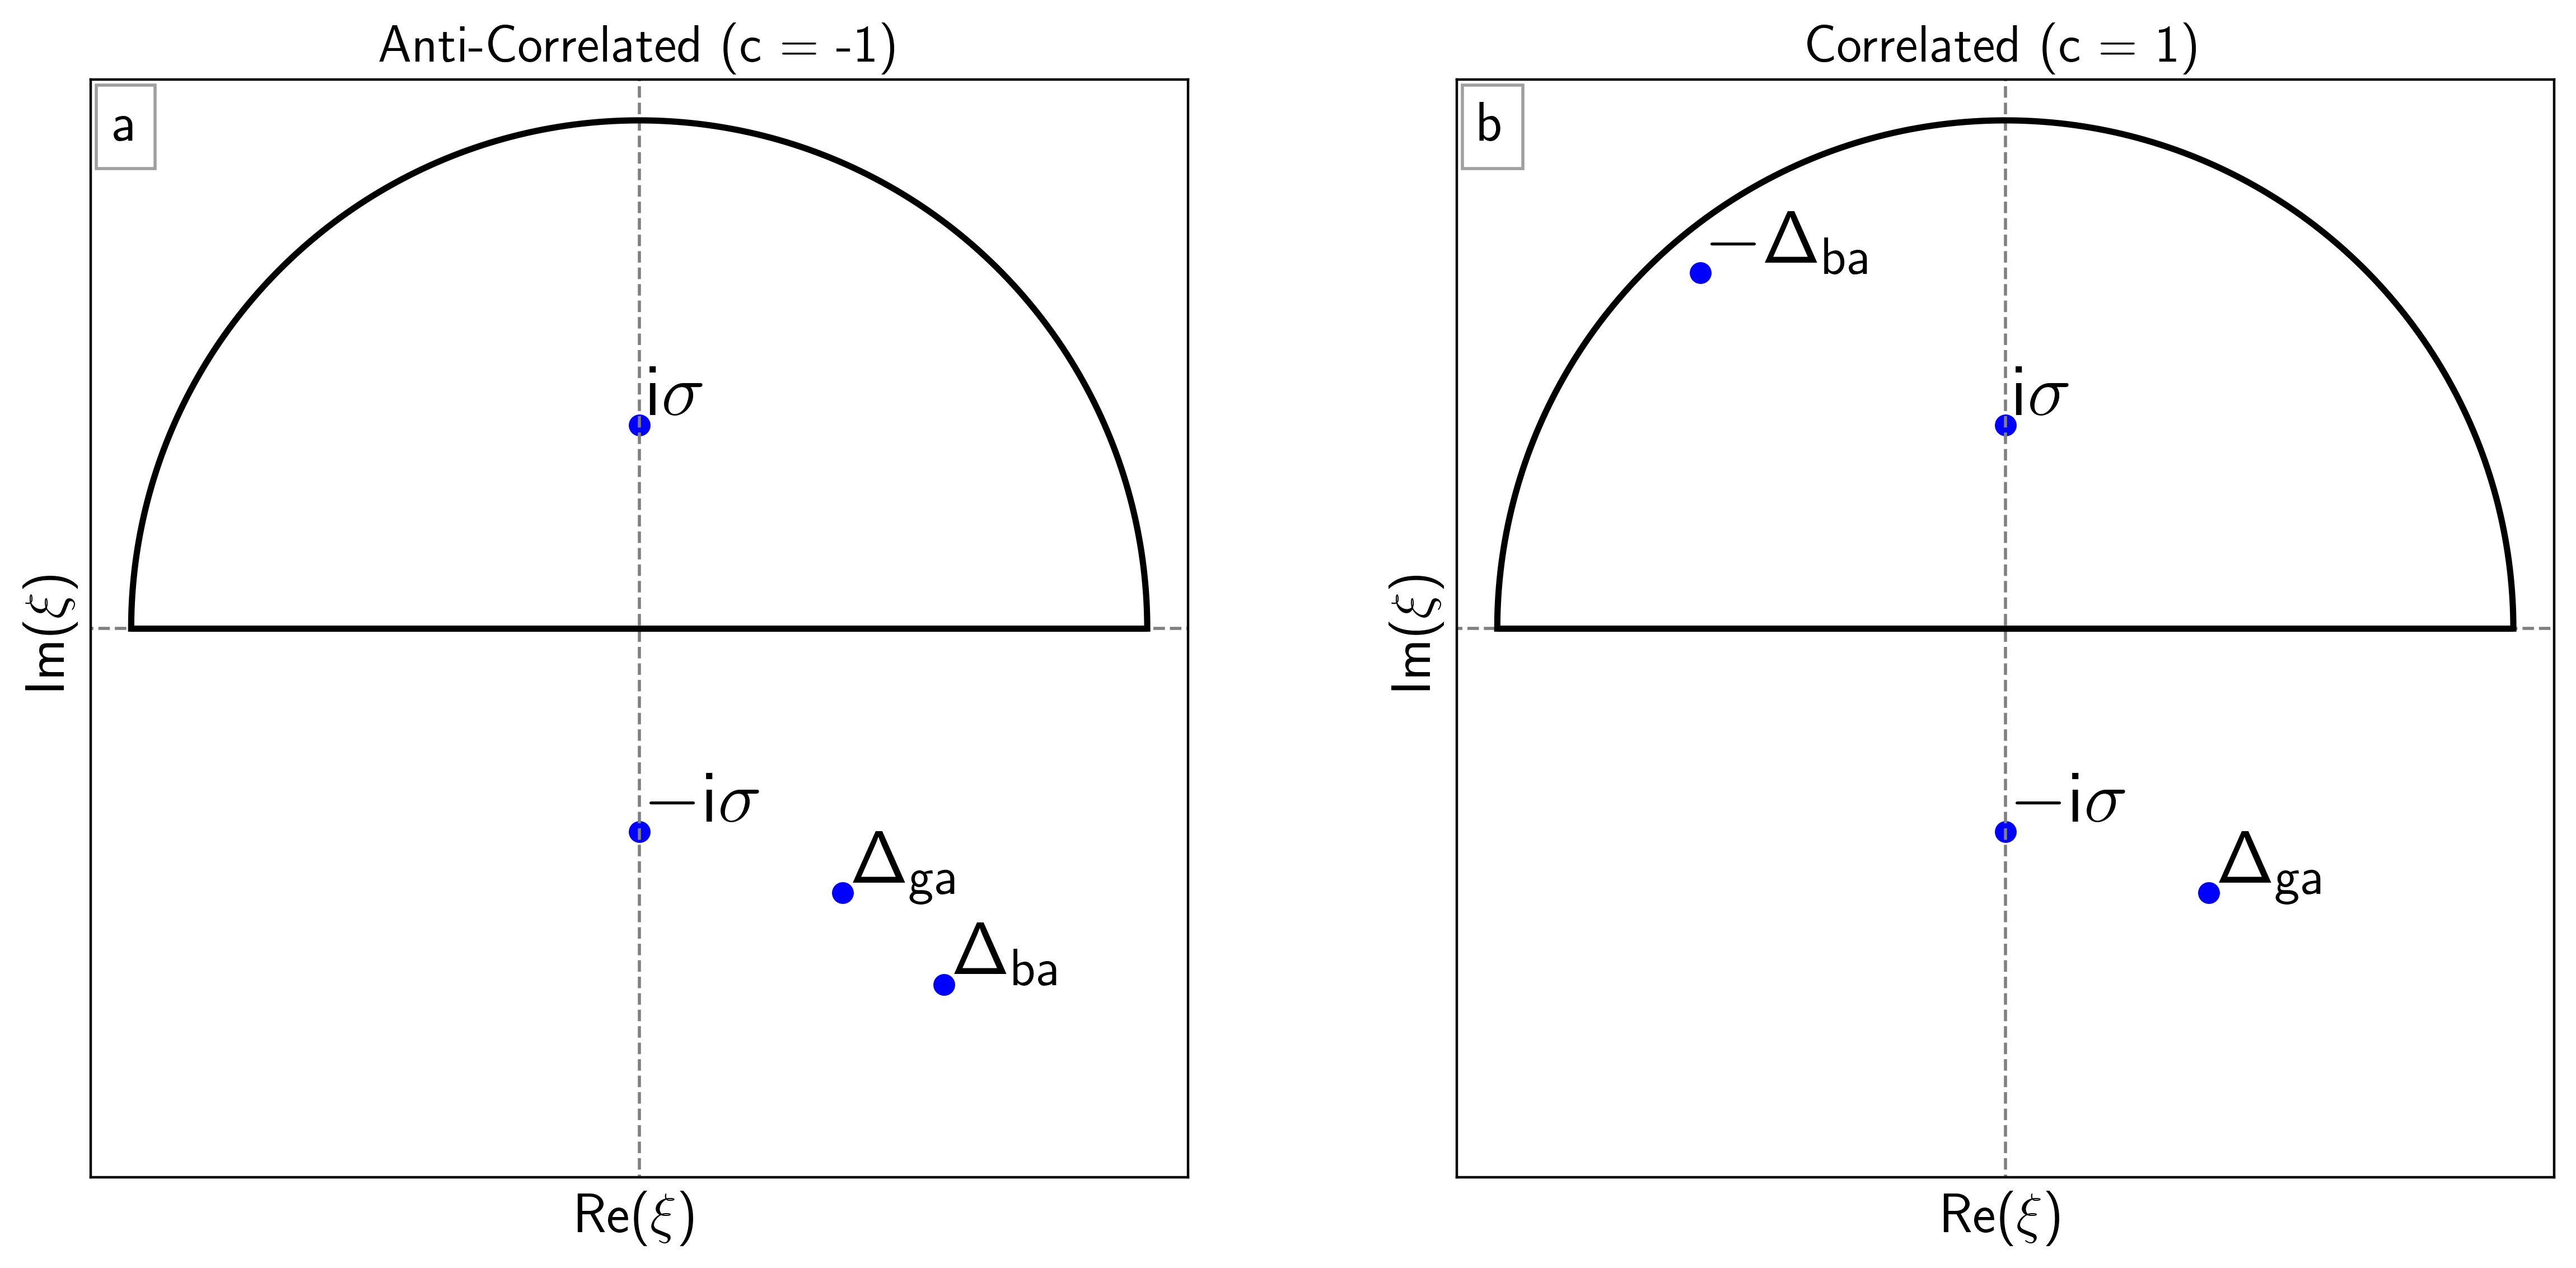
\includegraphics[width=3.375in]{figures/corr_contour.png}
	\caption{Poles (black dots) and contour (blue line) used to evaluate \autoref{integraly} for (a) anti-correlated and (b) correlated modes.} 
	\label{fig:contours}
\end{figure}
\subsubsection{Anti-correlated Modes}
For anti-correlated modes, the poles are situated in the complex plane as shown in \autoref{fig:contours}a.
Since \autoref{integraly} is evaluated along the real axis, one can choose to evaluate the contour in the upper or lower half of the complex plane.
Since evaluating the residues in the upper or lower half of the complex plane yields the same result for \autoref{integraly}, we choose the contour which wraps around the least number of poles.
It is clear for c = -1 that there are four poles: $\pm i \sigma, \Delta_{ga}(0), \Delta_{ba}(0)$. 
Following \autoref{fig:contours}, the contour that wraps the upper half of the complex plane has only one pole, $i \sigma$; as such, we choose to evaluate \autoref{integraly} in the upper half of the complex plane for the case of anti-correlated modes through the residue theorem as
\begin{widetext}
	\begin{equation}
		\begin{split}
			\rho_{ba} = \int_{-\infty}^\infty \mathrm{d}\xi P(\xi) \rho_{ba}(\xi) &= 2\pi i \sum_k \lim_{\xi \rightarrow \xi_k} P(\xi) \rho_{ba}(\xi) (\xi - \xi_k)\\
			&= 2\pi i \frac{\eta \sigma}{\pi} \lim_{\xi \rightarrow i\sigma} \frac{1}{(\xi + i\sigma)(\xi - i\sigma)} \frac{1}{\Delta_{ga}(0) - \xi} \frac{1}{\Delta_{ba}(0) - \xi} (\xi - i \sigma)\\
			&= 2 \eta \sigma i \lim_{\xi \rightarrow i\sigma} \frac{1}{\xi + i\sigma} \frac{1}{\Delta_{ga}(0) - \xi} \frac{1}{\Delta_{ba}(0) - \xi}\\
			&= 2\eta \sigma i \frac{1}{2i\sigma} \frac{1}{\Delta_{ga}(0) - i\sigma} \frac{1}{\Delta_{ba}(0) - i\sigma}\\
			&= \frac{\eta}{\Delta_{ga}(i\sigma)\Delta_{ba}(i \sigma)}\\
		\end{split}
	\end{equation}
\end{widetext}
In words, we see the inhomogeneous envelope width $\sigma$ is added to the linewidth of each resonance (e.g., $\Gamma_{ag} \rightarrow \Gamma_{ag} + \sigma$).
Therefore, pathway I-a cannot linenarrow anti-correlated modes. 
\subsubsection{Correlated Modes: c = 1}
For correlated modes, the poles are situated in the complex plane as shown in \autoref{fig:contours}.
It is clear that no matter which contour is chosen, there is a contribution to the final integral from either $\Delta_{ba}(0)$ or $\Delta_{ga}(0)$. 
For the below calculation, we choose to evaluate along the contour in the bottom half of the complex plane, i.e., the poles ($\xi_k$) are $-i\sigma, \Delta_{ga}$.
We stress that since the integral is evaluated over $\mathbb{R}$ and there are no degenerate poles, the results below can be obtained by evaluating the contour which wraps around the poles $i\sigma, \Delta_{ba}$. 
Since the $\xi_k$ are nondegenerate, \autoref{integraly} can be evaluated using the Residue theorem as 
\begin{widetext}
	\begin{equation}
		\begin{split}
			\int_{-\infty}^\infty \mathrm{d}\xi P(\xi) \rho_{ba}(\xi) &= 2\pi i \sum_k \lim_{\xi \rightarrow \xi_k} P(\xi) \rho_{ba}(\xi) (\xi - \xi_k)\\
			&= 2\pi i \frac{\eta \sigma}{\pi} ( \lim_{\xi \rightarrow -i\sigma} \frac{1}{(\xi + i\sigma)(\xi - i\sigma)} \frac{1}{\Delta_{ga}(0) - \xi} \frac{1}{\Delta_{ba}(0) - \xi} (\xi + i \sigma) \\ &+
			\lim_{\xi \rightarrow \Delta_{ga}(0)} \frac{1}{(\xi + i\sigma)(\xi - i\sigma)} \frac{1}{\Delta_{ga}(0) - \xi} \frac{1}{\Delta_{ba}(0) - \xi} (\xi - \Delta_{ga}))\\
			&= 2 \eta i \sigma (\frac{1}{2 i \sigma} \frac{1}{-i \sigma - \Delta_{ga}(0)} \frac{1}{\Delta_{ba}(0) - i\sigma} ) - 2 \eta i \sigma (\frac{1}{\sigma^2 + (\Delta_{ga} (0))^2} \frac{1}{\Delta_{ga}(0) + \Delta_{ba}(0)} )\\
			&= -\frac{\eta}{\Delta_{ga}(0) + i \sigma} (\frac{1}{\Delta_{ba}(0) - i \sigma} + \frac{2i\sigma}{(\Delta_{ga}(0) - i \sigma)(\Delta_{ga}(0) + \Delta_{ba}(0))})\\
		\end{split}
	\end{equation}
\end{widetext}
The final line of the above equation shows the presence of a new term, $\frac{2i\sigma}{\Delta_{ga}(0) + \Delta_{ba}(0)}$. 
This term is amplified by the width of the inhomogeneous envelope ($\sigma$) and has a linewidth $\Gamma_{ba} + \Gamma_{ga}$, which linenarrows the transition. 
Results for the other pathways follow the same technique.
Generally, when starting from the ground state, non-parametric spectroscopies line-narrow correlated modes, and parametric spectroscopies line-narrow anti-correlated modes. \cite{Dick83_1, RN425}


\section{References}
% Create the reference section using BibTeX:
\bibliography{library.bib}

\end{document}
%


